\chapter{Numerical Modeling}
\label{ch:numerical}
%
\par Coronal loop modeling can be roughly divided into two categories: multi-dimensional (typically 3D) magnetohydrodynamic models and hydrodynamic models. The former focuses primarily on the study of the dynamics of the magnetic field itself; the latter concentrates on the response of the plasma for some \textit{ad-hoc} heating and prescribed, static field geometry \citep{bradshaw_influence_2013}. While a hydrodynamic treatment may seem overly simplified, such models often provide a much more physically realizable treatment of the plasma than most 3D MHD models. This thesis will examine primarily the use of hydrodynamic models in the study of coronal plasma dynamics. By using hydrodynamic models, the evolution and response of the plasma to various heating functions can be carefully treated. In particular, this work will focus on the role of a two-fluid treatment in efficient hydrodynamic simulations. Such efficient models allow for the exploration of large parameter spaces with comparably little computational overhead.
%
\section{One-dimensional Two-fluid Hydrodynamics}
\label{sec:1dhydro}
%
\par In \S\ref{subsec:hydro}, the hydrodynamic equations were discussed under the assumption that the electron and ion populations were in equilibrium at all times (i.e. a single-fluid approximation). However, since the mechanism behind coronal heating is still highly debated, the degree to which the ions or electrons are preferentially heated is unknown. It is often assumed that the electrons are the direct recipients of the prescribed heating function. However, it is also possible that the ions are preferentially heated. One particular example is that of ion-cyclotron wave resonances \citep{markovskii_intermittent_2004}. Ion cyclotron waves are excited by plasma instabilities in the lower corona. These waves then propagate upwards through the coronal plasma and wave particle interactions can occur for those ions whose gyrofrequencies have a resonance with the ion-cyclotron wave. Additionally, there is also evidence for ion heating via reconnection, both in laboratory plasmas and particle-in-cell simulations \citep{ono_ion_1996,yoo_bulk_2014,drake_onset_2014}. Thus, ion heating in the solar corona should not be discounted as a possibility.
%
\par In this work, quasi-neutrality, $n_e=n_i=n$, will be assumed. While the heavier ions are in higher charge states and have thus given up more than one electron per ion, $\mathrm{Ab}_{\mathrm{H}}\gg\mathrm{Ab}_{X>\mathrm{H}}$. In other words, the abundance of (singly ionized) H is so much greater than the multiply-ionized heavier elements that quasi-neutrality is a valid assumption. Additionally, current-free conditions are also assumed such that $v_e=v_i=v$. Under these assumptions, the conservative forms of the mass and momentum equations can be written,
\begin{align}
	\frac{\partial\rho}{\partial t} &= -\frac{\partial(\rho v)}{\partial s} \label{eq:1dmass}, \\[0.5em]
	\frac{\partial(\rho v)}{\partial t} &= -\frac{\partial(\rho v^2)}{\partial s}-\frac{\partial(p_e + p_i)}{\partial s} + \frac{\partial}{\partial s}\left(\frac{4}{3}\mu_i\frac{\partial v}{\partial s}\right) + \rho g_{\parallel}, \label{eq:1dmom}
\end{align}
where $\rho=m_en_e + m_in_i=n(m_e+m_i)\approx nm_i$, $m_i$ is the ion mass, $p_e$ and $p_i$ are the electron and ion pressures respectively, and $\mu_i=m_iu_i$, where $u_i$ is the classical Spitzer viscosity coefficient \citep{bradshaw_influence_2013}. Notice that Eq. \ref{eq:1dmass} is equivalent to its single-fluid counterpart due to our assumption of quasi-neutrality and that the only difference between Eq. \ref{eq:1dmom} and Eq. \hl{SF MOM EQ REF HERE} is the addition of the ion viscosity term and that $p=p_e+p_i$.
%
\par The electron and ion energy equations are given by
\begin{align}
	\frac{\partial E_e}{\partial t} &= -\frac{\partial}{\partial s} \lbrack(E_e+p_e)v\rbrack+v\frac{\partial p_e}{\partial s} - \frac{\partial F_{e}}{\partial s} + \frac{1}{\gamma - 1}k_Bn\nu_{ei}(T_i-T_e) -E_R+E_{H,e}, \label{eq:1denergy_e} \\[0.5em]
	\frac{\partial E_i}{\partial t} &= -\frac{\partial }{\partial s}\lbrack(E_i+p_i)v\rbrack-v\frac{\partial p_e}{\partial s} - \frac{\partial F_{i}}{\partial s} + \frac{1}{\gamma - 1}k_Bn\nu_{ei}(T_e-T_i) + \frac{\partial}{\partial s}\left(\frac{4}{3}\mu_iv\frac{\partial v}{\partial s}\right) +\rho v g_{\parallel} + E_{H,i},\label{eq:1denergy_i}
\end{align}
where $E_e$ and $E_i$ are the electron and ion energies, respectively, and $E_{H,e}$ and $E_{H,i}$ are the \textit{ad-hoc} volumetric heating rates for the electrons and ions, respectively. Furthermore, this set of equations is subject to the closure conditions
\begin{align}
	E_e = \frac{p_e}{\gamma - 1}, \label{eq:ee_close} \\[0.5em]
	E_i = \frac{p_i}{\gamma - 1} + \frac{1}{2}\rho v^2, \label{eq:ei_close} \\[0.5em]
	p_e = k_BnT_e, \label{eq:pe_close} \\[0.5em]
	p_i = k_BnT_i, \label{eq:pi_close}
\end{align}
where $\gamma=5/3$ is the adiabatic index.
% 
\par The conductive heat fluxes for the ions and electrons, $F_e$ and $F_i$, are given by the classical Spitzer-Harm \citep{spitzer_transport_1953} formulas
\begin{align}
	F_e=-\kappa_{0,e}T_e^{5/2}\frac{\partial T_e}{\partial s}, \label{eq:1dhfluxe} \\[0.5em]
	F_i=-\kappa_{0,i}T_i^{5/2}\frac{\partial T_i}{\partial s}, \label{eq:1dhfluxi}
\end{align}
where $\kappa_{0,e}$ and $\kappa_{0,i}$ are the Spitzer coefficients for electron and ion thermal conduction, respectively \citep{bradshaw_influence_2013}. The classical formula for the heat flux, however, is known to be inaccurate at high temperatures and low densities. To correct for this, a flux-limiter or free-streaming limit is often used, such that the heat flux saturates at
\begin{equation}
	F_{sat,s} = -\beta\frac{3}{2}\frac{k^{3/2}}{m_s^{1/2}}nT_s^{3/2},
\end{equation}
where $s$ specifies the particles species \citep{bradshaw_explosive_2006}. This prevents the heat flux from becoming unphysically large, particularly during the onset of heating when the temperature is high and the density relatively low. $\beta$ is a flux limiter constant with a typical value between $1$ and $1/6$ \citep{luciani_nonlocal_1983,karpen_nonlocal_1987}. The final expression for the conductive flux for species $s$ can then be written as
\begin{equation}
	F_s=\frac{F_{c,s}F_{sat,s}}{\sqrt{F_{c,s}^2 + F_{sat,s}^2}},
\end{equation}
where $F_{c,s}$ is the classical expression for the heat flux for species $s$ as given in Eqs. \ref{eq:1dhfluxe} and \ref{eq:1dhfluxi}. Thus, $F_s\approx F_{c,s}$ when $|F_{c,s}|\ll|F_{sat,s}|$ and $F_s\approx F_{sat,s}$ when $|F_{c,s}|\gg|F_{sat,s}|$.
%
\par The electron and ion energy equations are coupled through a collisional term proportional to the Coulomb collision frequency times the difference between the temperatures of the respective species. The Coulomb collision frequency is given by
\begin{equation}
	\nu_{ei} = \frac{16\sqrt{\pi}}{3}\frac{e^4}{m_em_i}\left(\frac{2k_BT_e}{m_e}\right)^{-3/2}n\ln{\Lambda},
\end{equation}
where $\ln{\Lambda}\approx20$ is the Coulomb logarithm. If the heating timscale is much greater than $1/\nu_{ei}$, the collisional timescale, then electron-ion equilibrium cannot be assumed during the heating phase. In particular, for $n\sim10^8~\mathrm{cm}^{-3}$ and $T\sim10^7~\mathrm{K}$, parameters typical of a nanoflare-heated coronal plasma, the collisional timescale can be estimated as $\tau_{ei,coll}\sim1/\nu_{ei}\approx8000$ s. So any heating occurring on a timescale less than 8000 s will force the electron and ion populations out of equilibrium. Often when modeling nanoflares, heating timescales of a few hundreds or even a few tens of seconds are used. Thus, treating the evolution of the electron and ions separately is particularly important when studying impulsive heating in coronal loops.
%
\section{``0''-Dimensional Hydrodynamic Models }
\label{sec:0dmodels}
%
\par As discussed in \S\ref{sec:1dhydro} and \S\ref{subsec:hydro}, 1D hydrodynamic models are an invaluable tool for studying the plasma dynamics of the solar corona. However, while these models only consider evolution in the field-aligned direction, their solutions still necessitate a careful treatment of several highly-nonlinear partial differential equations. Perhaps the greatest restriction imposed on these models is the need to resolve the thermal conduction timescale, given by $\Delta t_C=4\times10^{-10}n\Delta s^2/T^{5/2}$. For a transition region plasma with an adequate grid size, this can result in a timestep on the order of several milliseconds \citep{bradshaw_influence_2013}. This makes modeling events in excess of a few hours tedious and computing thousands of field lines nearly impossible. Additionally, as 1D hydrodynamic codes become more sophisticated, incorporating features such as adaptive mesh refinement and effects due to non-equilibrium ionization, their output becomes increasingly more complicated and difficult to interpret \citep{cargill_enthalpy-based_2012-1}.
%
\par Thus, there is a need for codes which a) provide an efficient way to model dynamic coronal loops and b) generate output that provides physical insight into the evolution of the plasma and the resulting physical observables. Zero-dimensional or ``0D'' hydrodynamic models satisfy both of these requirements. 0D models have long been used as a tool to better understand static and dynamic coronal loop configurations. They provide a way to efficiently compute loop parameters such as $T$ and $n$ while incorporating the plasma processes known to be dominant in coronal loops. Most 0D loop models compute spatially-averaged time-dependent quantities and thus provide a way to perform large parameter-space surveys in reasonable amounts of time while relaxing the static equilibrium assumption.
%
\par The scaling laws of \citet{rosner_dynamics_1978} are often considered some of the first 0D models as they provided simple expressions for relating the loop length, temperature, pressure, and heating rate. However, these analytic models did not provide a way to analyze loop dynamics. In the last thirty years, several 0D models have attempted to provide efficient ways to model loop dynamics. These include, but are not limited to, \citet{fisher_equation_1990,kopp_coronal_1993,cargill_implications_1994,aschwanden_hydrodynamic_2009}. While many of these 0D models provided good insight into different regimes of loop evolution, \citet{cargill_enthalpy-based_2012-1} show that each of these approaches has significant drawbacks when one considers the evolution of the loop throughout an entire cycle of heating and cooling. In particular, many do not treat the conductive and radiative cooling regimes correctly, do not allow for a generalized heating function, and/or do not carefully take into account the coupling between the corona and transition region. 
%
\par\hl{Discuss importance of two-fluid effects in hydrodynamic models of the solar corona; include some quick calculations to show how electron and ion fluids can become decoupled}
\hl{If there is time, discuss speed comparison between EBTEL and HYDRAD}
%
\subsection{The EBTEL Model}
\label{subsec:ebtel}
%
\par The Enthalpy-Based Thermal Evolution of Loops (EBTEL) model \citep{klimchuk_highly_2008,cargill_enthalpy-based_2012} was developed initially to study nanoflare heating, but can handle a generalized heating input. EBTEL divides the loop into coronal and transition region parts, where the boundary is defined by the location at which thermal conduction switches from a source term (transition region) to a loss term (corona). The basic idea behind EBTEL, as the name implies, is to equate an enthalpy flux with any difference in magnitude between the conductive heat flux and the radiative losses from the transition region \citep{klimchuk_highly_2008}. In this way, the processes of evaporation and condensation, the filling and draining of the coronal portion of the loop, can be accurately modeled in a 0D context. 
%
\par The governing equations of the EBTEL model are derived by computing spatial averages over the coronal and transition region portions of the loop. In particular, spatial integrals of the 1D hydrostatic equations (see \S\ref{subsec:hydro}) are taken over the corona (length $L$) and the much thinner transition region (length $\ell\ll L$). EBTEL relies on several key assumptions: a) the flow is assumed to be subsonic, $v<C_s$, such that terms $\mathcal{O}(v^2)$ are ignored; b) the loop is shorter than a gravitational scale height such that gravitational terms are ignored; c) the ratios $c_2=\bar{T}/T_a$ and $c_3=T_0/T_a$, where $\bar{T},T_a,T_0$ are the coronally averaged, apex, and base temperatures, respectively, are fixed such that $c_2=0.9$ and $c_3=0.6$. Additionally, as is common in loop models, only one half of the loop is computed, with symmetry about the apex assumed \citep{klimchuk_highly_2008}.
%
\par The 0D EBTEL equations, as given by \citet{cargill_enthalpy-based_2012}, are
\begin{align}
	\frac{1}{\gamma - 1}\frac{d\bar{p}}{dt} = \bar{E_H} - \frac{\mathcal{R}_C}{L}(1+c_1), \label{eq:ebtel_sf_pressure} \\[0.5em]
	\frac{d\bar{n}}{dt} = -\frac{c_2(\gamma - 1)}{c_32k_B\bar{T}L\gamma}(F_0 + c_1\mathcal{R}_C), \label{eq:ebtel_sf_density}
\end{align}
where $\bar{n}$ and $\bar{p}$ are the coronally averaged density and pressure, respectively, $F_0$ is the heat flux at the base of the corona, $\mathcal{R}_C=\int_C\mathrm{d}s~E_R$ is the coronal spatial integral over the radiative loss term and $c_1=\mathcal{R}_{tr}/\mathcal{R}_c$ is the ratio between the spatially integrated radiative losses over the transition region and corona, respectively. Additionally, Eqs. \ref{eq:ebtel_sf_pressure} and \ref{eq:ebtel_sf_density} are closed by an equation of state, $\bar{p}=2\bar{n}k_B\bar{T}$, such that, given $\bar{n}$ and $\bar{p}$, the temperature $\bar{T}$ can be determined. It should be noted that \citet{klimchuk_highly_2008} determined that $c_1=4.0$ through an empirical method based on 1D hydrodynamic simulations. \citet{cargill_enthalpy-based_2012} later improved on this assumption by adding corrections for gravity and an improved estimated during the radiative cooling phase.
%
\begin{figure}
	\centering
	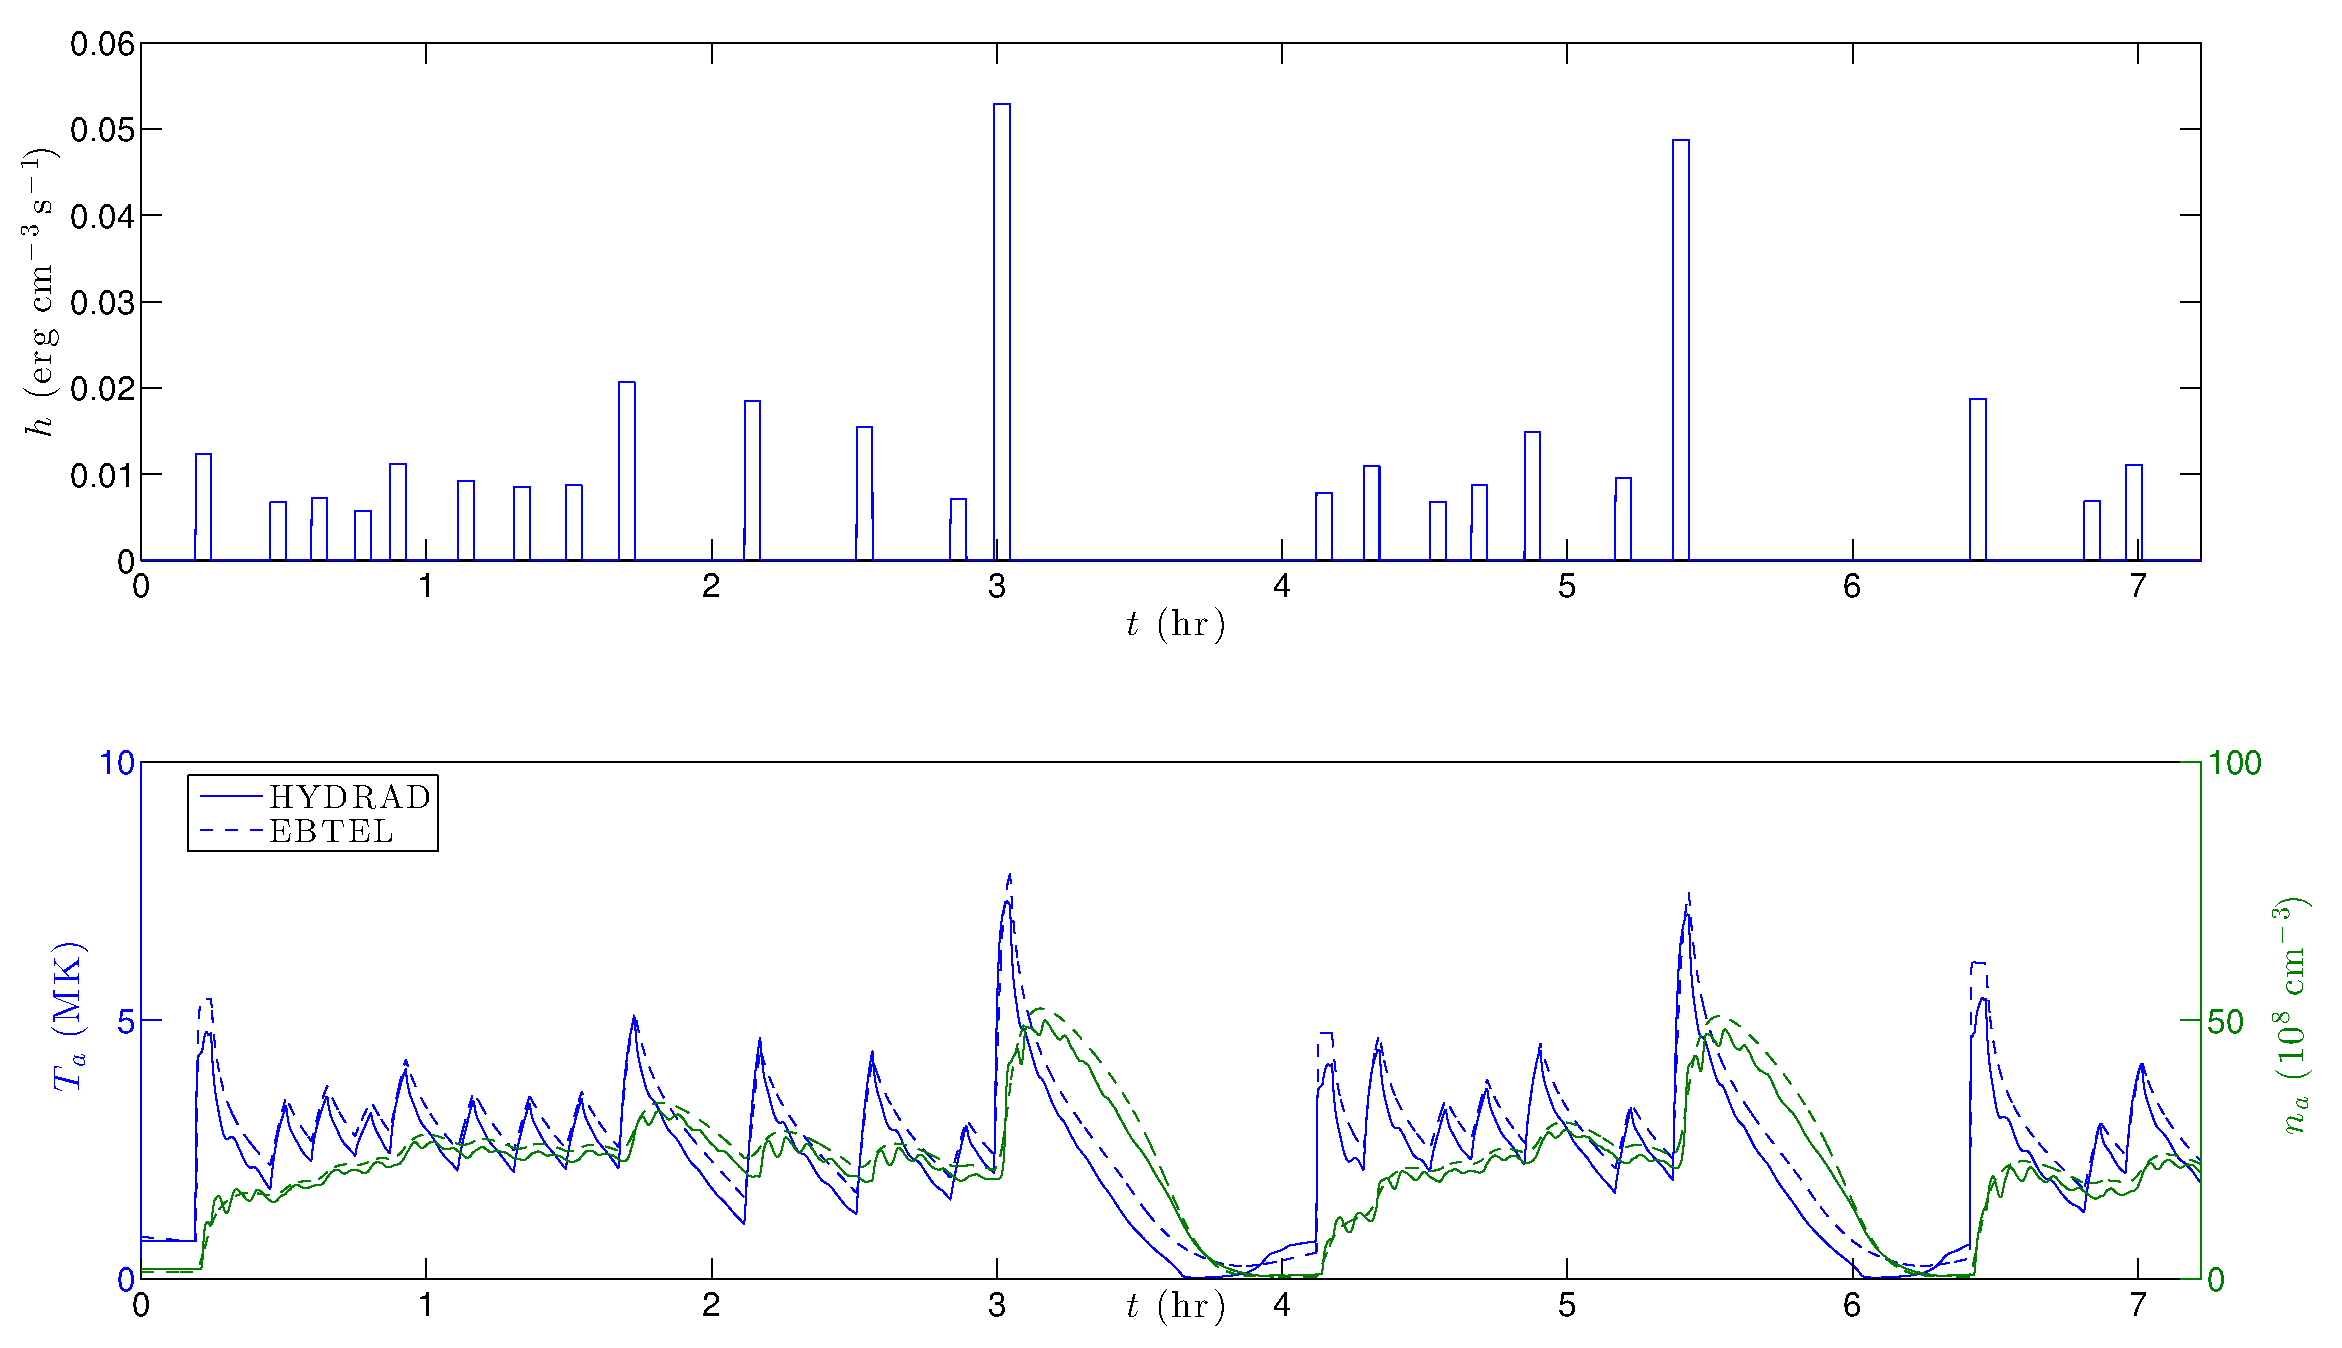
\includegraphics[width=0.95\textwidth]{figures/ebtel_sf_compare.eps}
	\caption{Comparison between EBTEL (dashed) and the 1D hydrodynamic code HYDRAD (solid) for a heating function with randomly chosen start times and amplitudes chosen from a power-law distribution. The upper panel shows the heating profile, the middle panel shows the temperature profiles, and the bottom panel shows the density profiles.For both the temperature and density, the EBTEL profile follows the HYDRAD profile quite closely. For the EBTEL profiles, the apex quantities are shown here. For the HYDRAD profiles, the quantities are averaged over the upper portion of the loop.}
	\label{fig:ebtel_sf_compare}
\end{figure}
%
\par EBTEL has been carefully benchmarked with the 1D hydrodynamic code HYDRAD. Fig. \ref{fig:ebtel_sf_compare} shows a comparison between EBTEL and HYDRAD for a series of impulsive, square heating events whose amplitudes are chosen from a power-law distribution. \citet{cargill_enthalpy-based_2012} also provide several comparisons between EBTEL and HYDRAD for triangluar, square, and gaussian heating pulses of varying duration and amplitude. Additionally, \citet{cargill_enthalpy-based_2012-1} show comparisons between EBTEL, HYDRAD, and earlier 0D models in an effort to show how EBTEL improves upon previous 0D efforts by matching 1D codes in both the initial heating and subsequent cooling phases of loop evolution.
%
\subsection{The Two-fluid EBTEL Model}
\label{subsec:two_fluid_ebtel}
%
\par\hl{Introduce EBTEL-2fl model by mentioning no two-fluid effects in EBTEL, refer back to previous section, derive equations, refer to figure}
%
\begin{figure}
	\centering
	\subfigure[]{%
	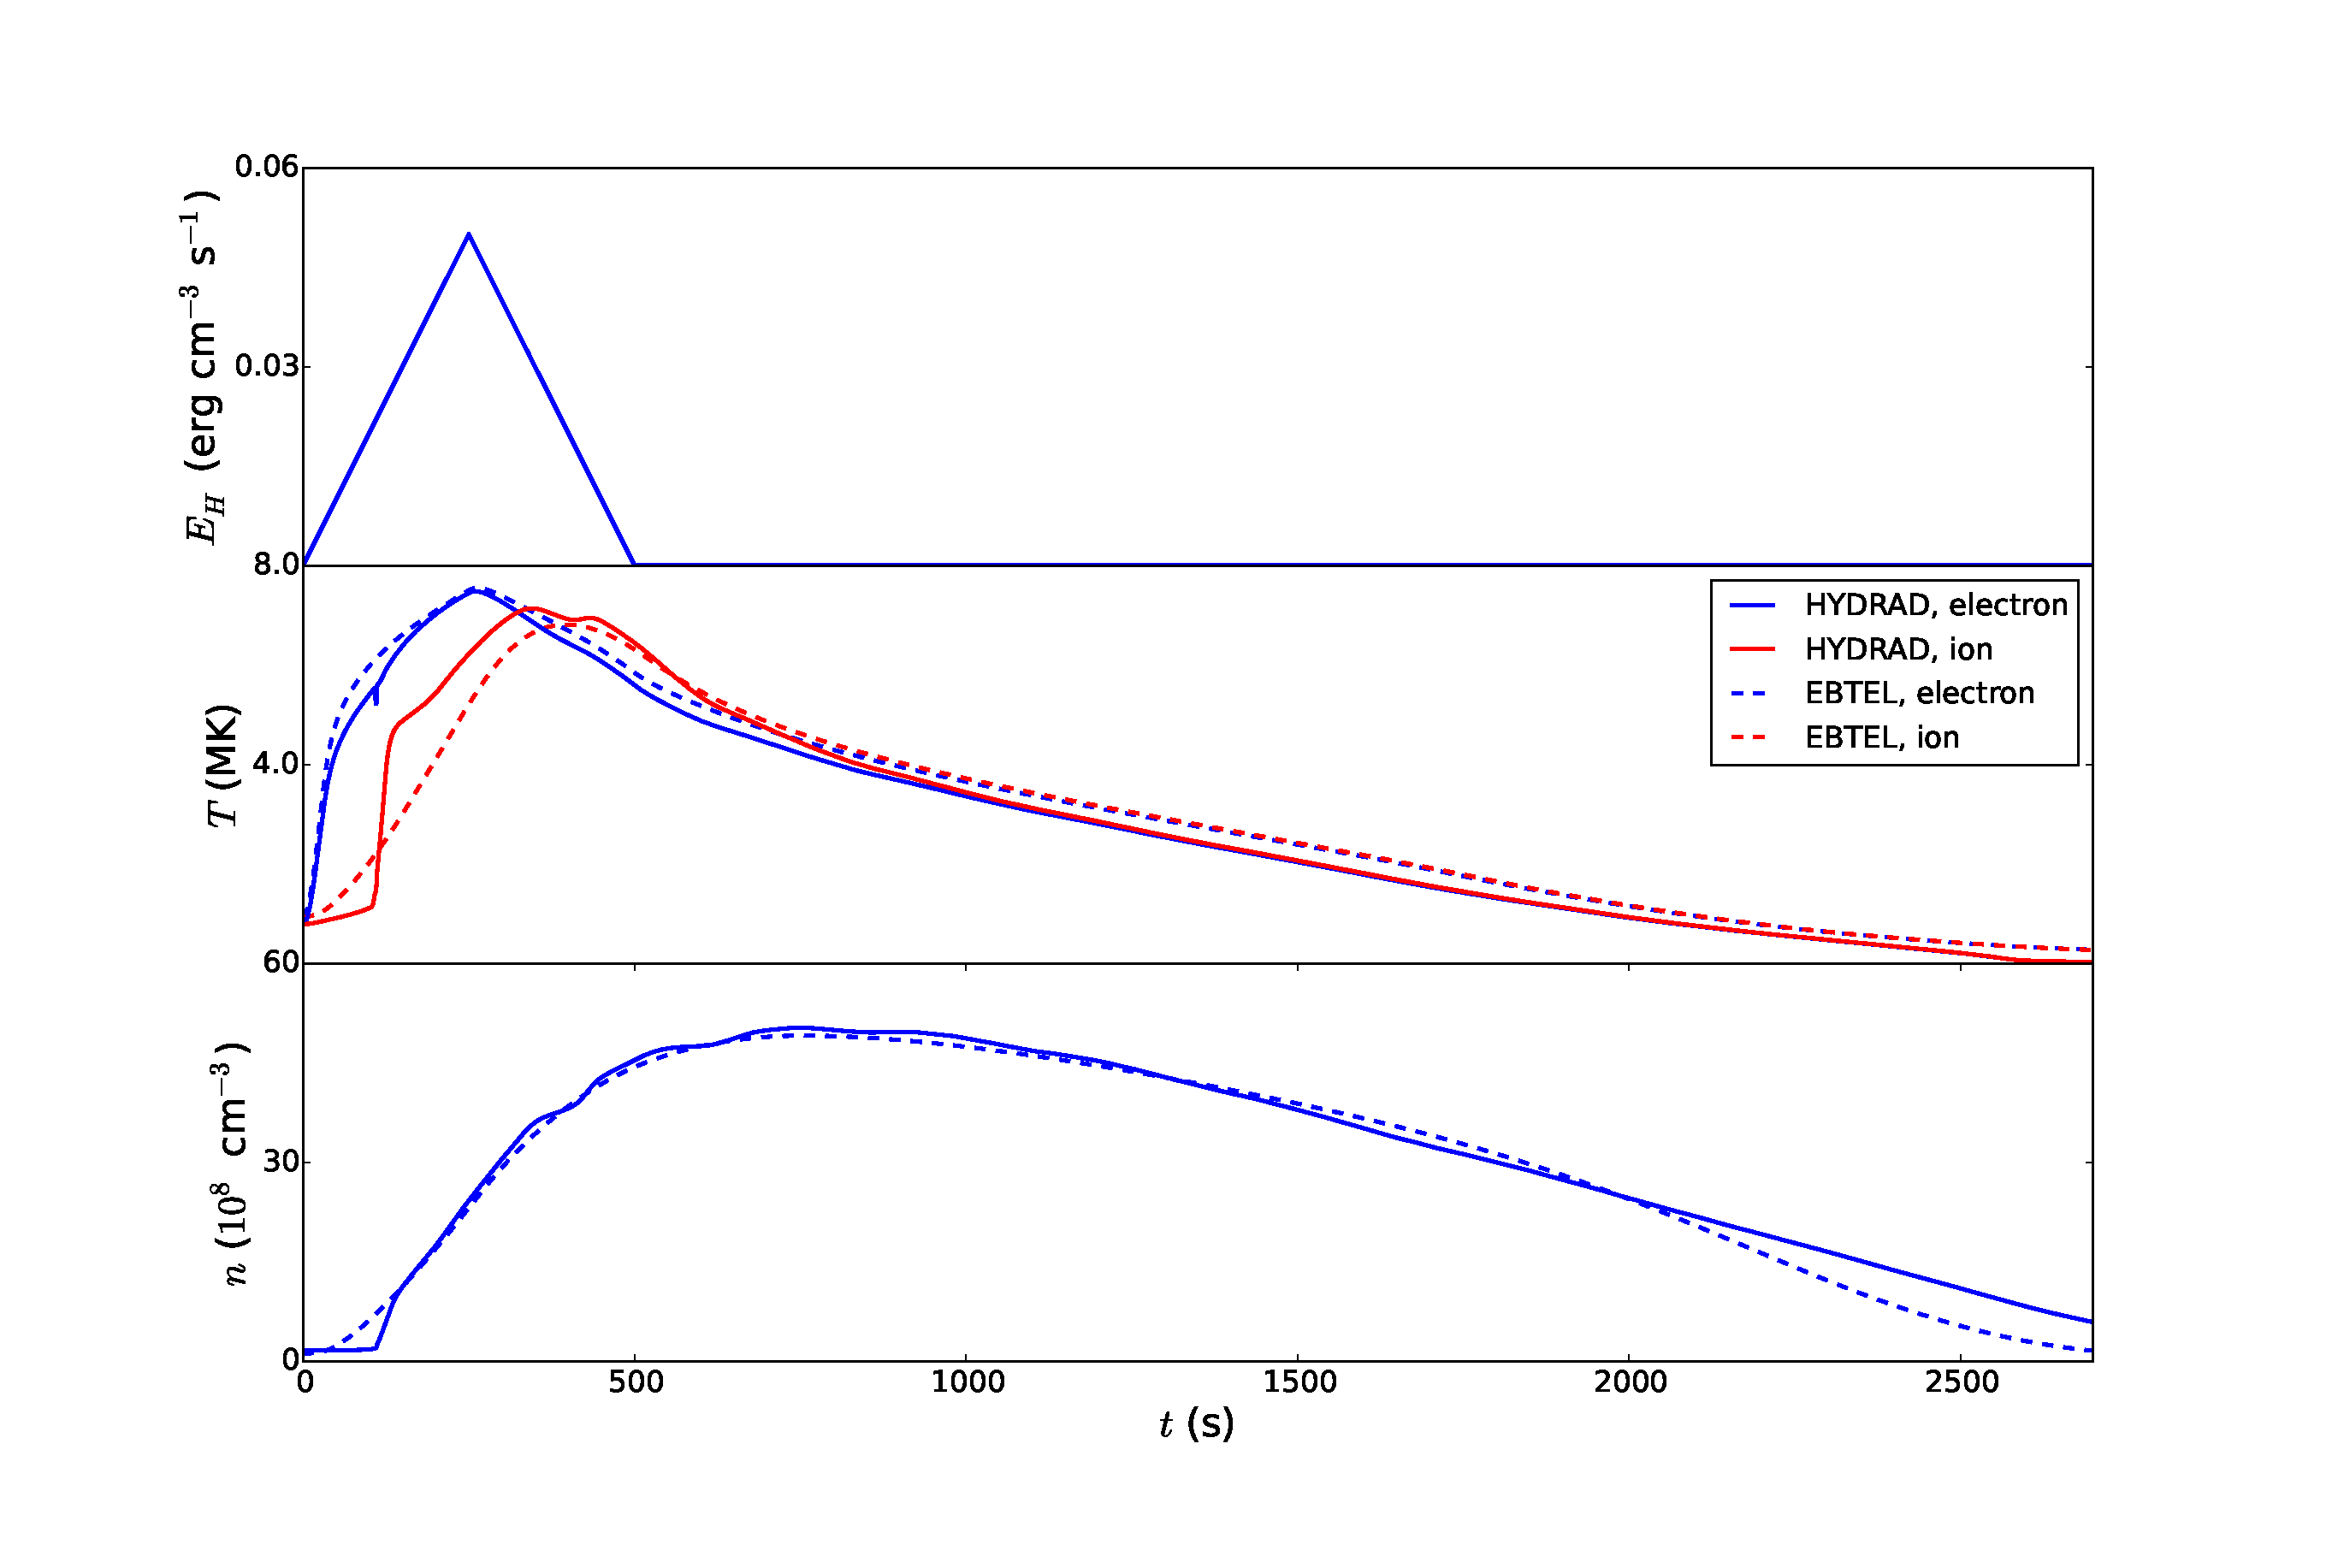
\includegraphics[width=0.85\textwidth]{figures/ebtel_tf_compare_1event.eps}
	\label{fig:ebtel_tf_compare_1}}
	\subfigure[]{%
	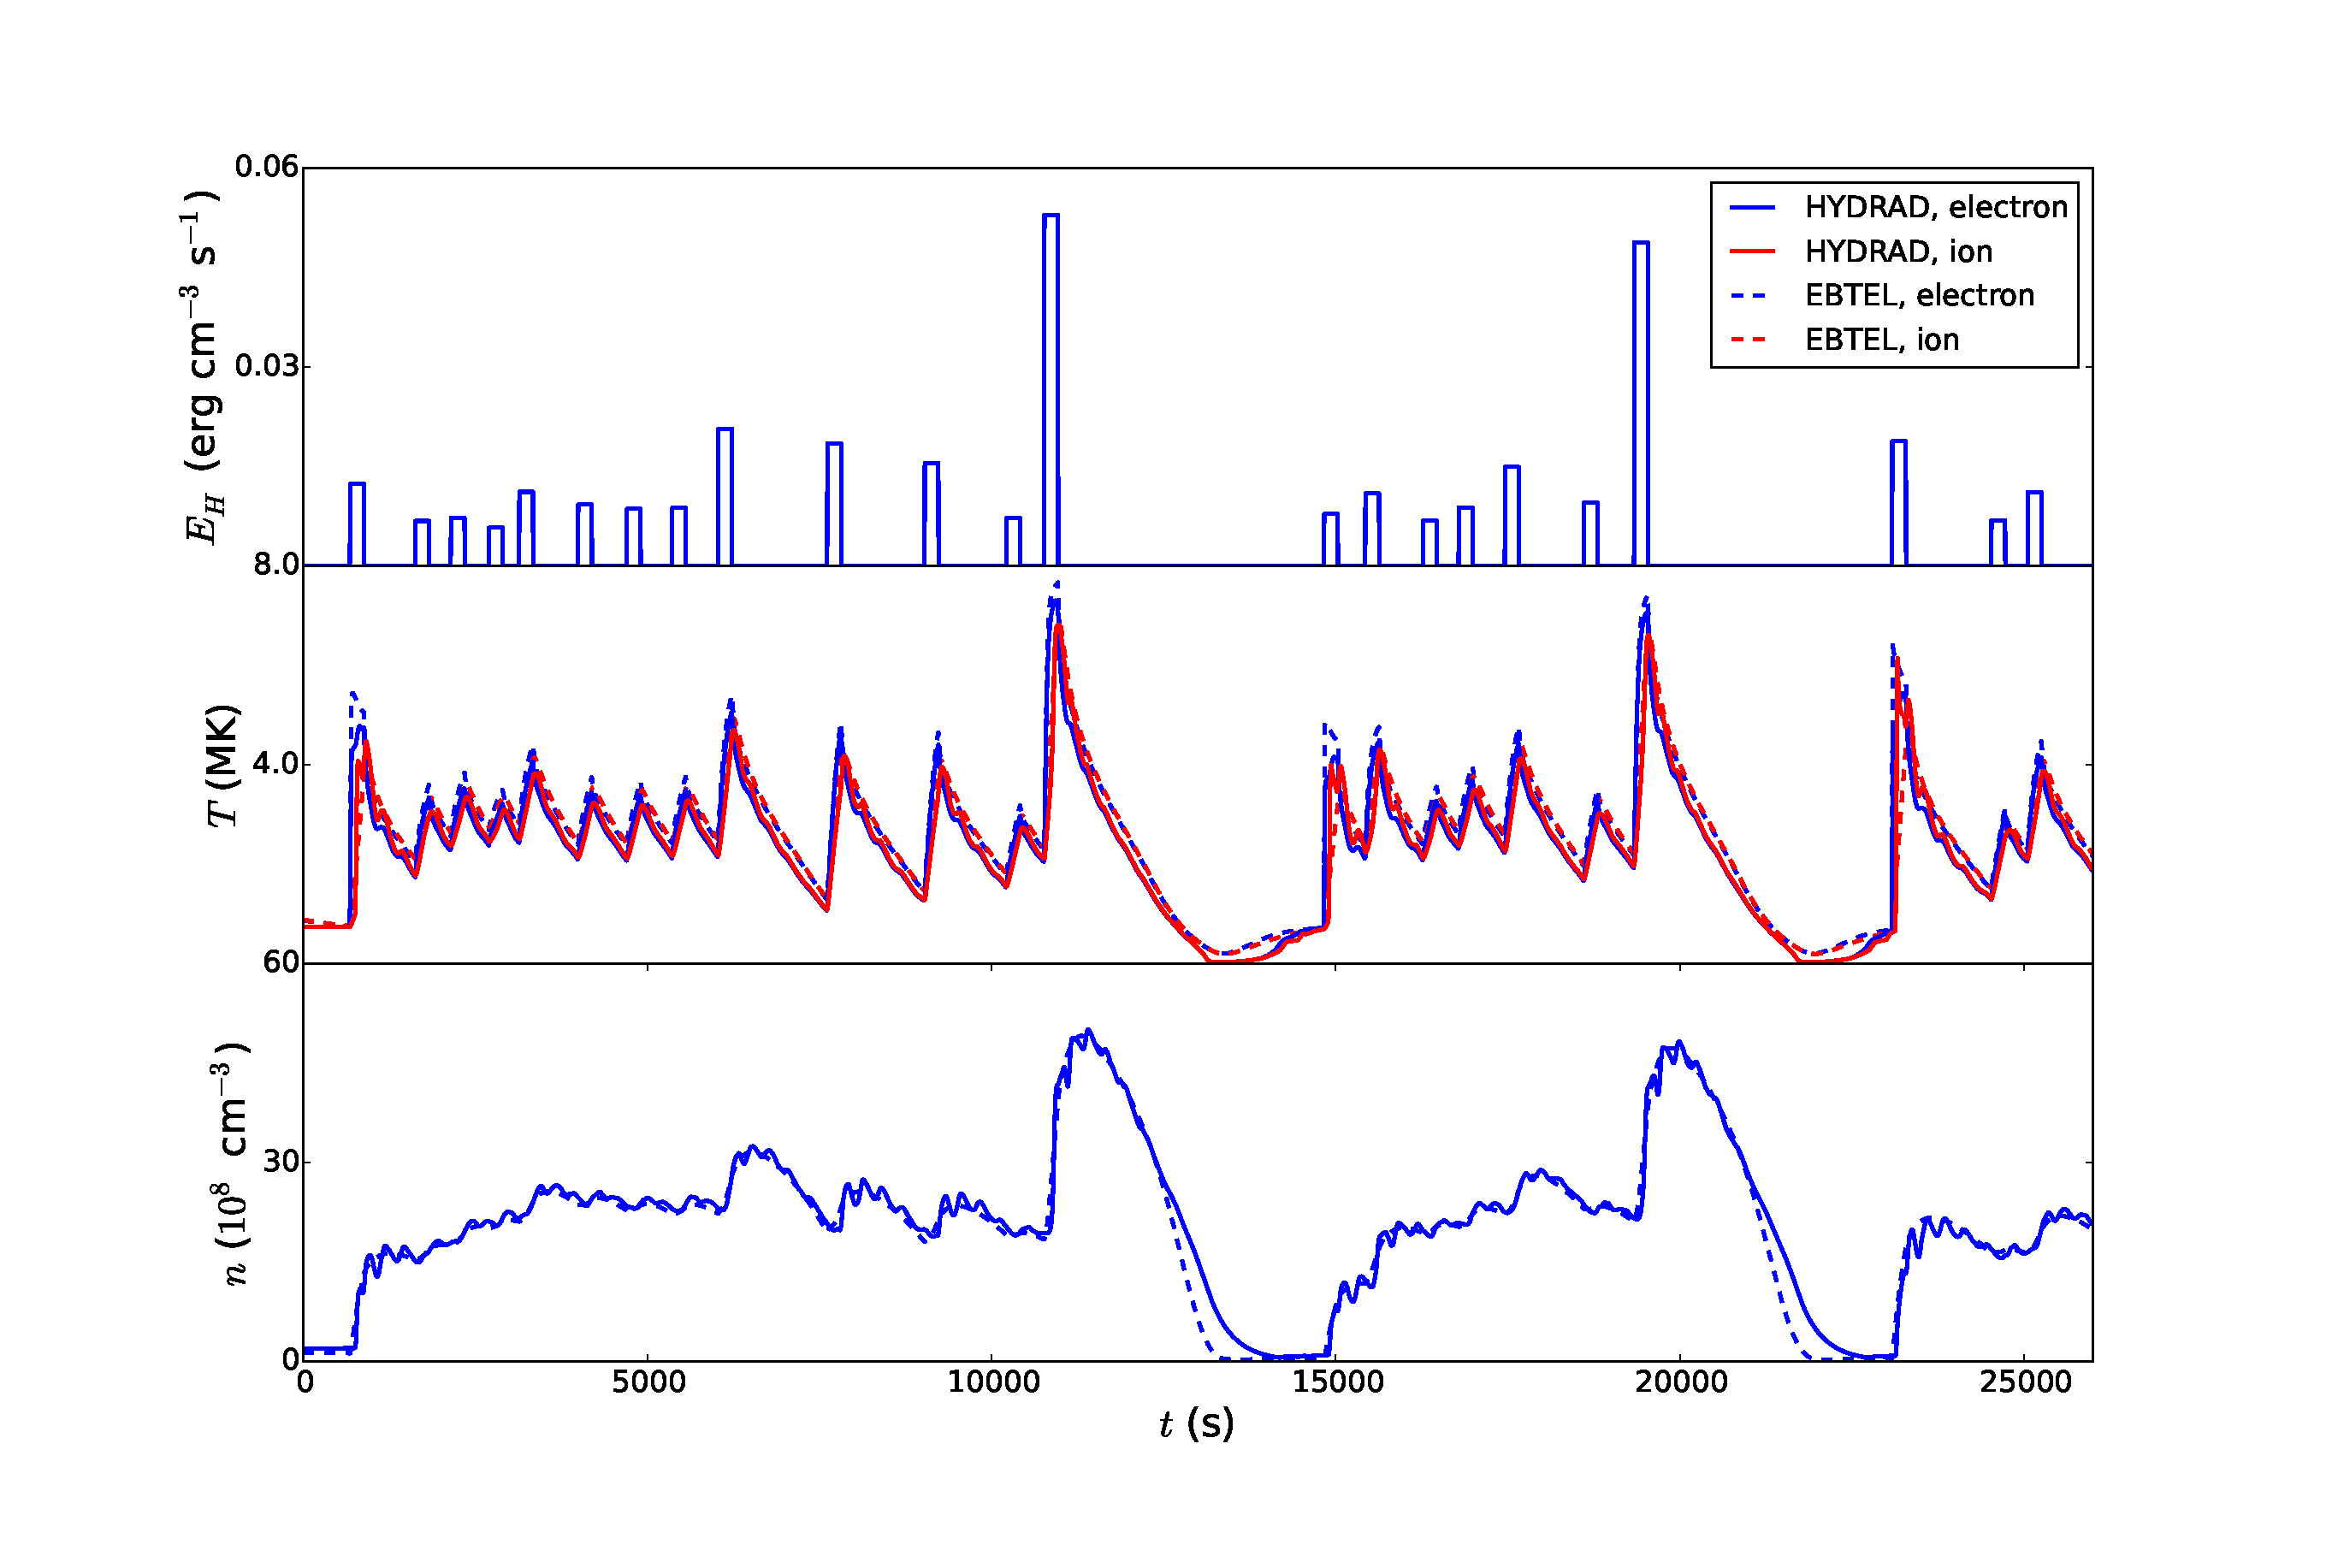
\includegraphics[width=0.85\textwidth]{figures/ebtel_tf_compare_manyevents.eps}
	\label{fig:ebtel_tf_compare_m}}
	\caption{Comparisons between the EBTEL-2fl model (dashed) and HYDRAD (solid) for \textbf{(a)} a single triangular pulse lasting 500 s and \textbf{(b)} the same heating profile as in Fig. \ref{fig:ebtel_sf_compare}. The upper panels show the heating profiles, the middle panels show the electron (blue) and ion (red) temperature profiles, and the bottom panels show the density profiles.}
	\label{fig:ebtel_tf_compare}
\end{figure}
%
\section{Numerical Implementation}
\label{sec:numerical}
%
\subsection{Euler Method}
\label{subsec:euler}
%
\subsection{Fourth-order Runge-Kutta Method}
\label{subsec:rk4}
%
\subsection{Adaptive Timestep Routine}
\label{subsec:adapt}
%